\documentclass[a4paper, 10pt]{article}

\usepackage[english]{babel}
\usepackage[T1]{fontenc}
\usepackage[utf8]{inputenc}
\usepackage{textcomp}
\setlength{\marginparwidth}{2cm}

\usepackage{comment}
\usepackage{todonotes}

\usepackage{amsmath}
\usepackage{amssymb}

\usepackage{enumitem}
\usepackage{array}
\setlength\extrarowheight{5pt}

\usepackage{xcolor}
\usepackage{graphicx}
\graphicspath{ {./img/} }

\usepackage{hyperref}
\usepackage{listings}
\usepackage{color}
\definecolor{dkgreen}{rgb}{0,0.6,0}
\definecolor{gray}{rgb}{0.5,0.5,0.5}
\definecolor{mauve}{rgb}{0.58,0,0.82}
\lstset{frame=tb,
    language=Python,
    aboveskip=3mm,
    belowskip=3mm,
    showstringspaces=false,
    columns=flexible,
    basicstyle={\small\ttfamily},
    numbers=none,
    numberstyle=\tiny\color{gray},
    keywordstyle=\color{blue},
    commentstyle=\color{dkgreen},
    stringstyle=\color{mauve},
    breaklines=true,
    breakatwhitespace=true,
    tabsize=3
}

\title{Homework Assignment N°4}
\author{BML36\\Thibault Douzon\\Rajavarman Mathivanan}
\date{September 26th, 2018}

\begin{document}
\maketitle

\pagebreak

\tableofcontents

\pagebreak
\section{Exercise 1: Decision Trees}
\subsection{Part a}
\paragraph{a}
Entropy of a particular class $x$ inside a dataset is given by the following formula:
$$
H(x) = -p(x)\ln_2(p(x))
$$
Where $\ln_2$ is the base 2 logarithm and $p(x)$ is the proportion of $x$ inside the dataset.
\\
In our case, $p(x) = \frac{4}{9}$, thus
$$
H(x_\text{+}) = -p(x_\text{+})\ln_2(p(x_\text{+})) = -\frac{4}{9}\ln_2(\frac{4}{9}) \approx 0.520
$$
\paragraph{b}
First let's compute the entropy of the dataset:
$$
H_0 = \sum_{i \in C^\text{target}} -p(i)\ln_2(p(i)) = -p(x_\text{+})\ln_2(p(x_\text{+})) -p(x_\text{-})\ln_2(p(x_\text{-}))
\approx 0.520 + 0.471 = 0.991
$$
The entropy of the whole dataset is $0.991$

Now we can look at feature $a_1$ and the repartition of its value accross the target class.
\\
We will use the same method as in the lectures, a  where each row represents a possible value
for the feature $a_1$ and the two firsts column give the number of elements, the two following the probabilities 
and the last one the entropy for this value.
\begin{center}
    \begin{tabular}{ |c|c|c|c|c|c| }
        \hline
        Feature $a_1$ & +      & -     & $p_\text{+}$ & $p_\text{-}$ & entropy\\
        \hline 
        T          & $3$    & $1$   & $\frac{3}{4}$ & $\frac{1}{4}$ & $0.811$\\
        \hline
        F          & $1$    & $4$   & $\frac{1}{5}$ & $\frac{4}{5}$ & $0.722$\\
        \hline
    \end{tabular}
\end{center}
We can now compute the mean entropy if we split on $a_1$:
$$
H_{a_1} = \sum_{i \in C^{a_1}} p(i)H(i_\text{+}, i_\text{-}) \approx \frac{4}{9}\times0.811 + \frac{5}{9}\times0.722 \approx 0.762
$$
The new entropy if we slit on $a_1$ is $0.762$
\\
We can now compute the information gain:
$$
IG(a_1) = H_0 - H_{a_1} \approx 0.991 - 0.762 \approx 0.229
$$
The information gain on splitting on $a_1$ is $0.229$

We apply the same method to compute the information gain on splitting on $a_2$.
\\
We get the following :
\begin{center}
    \begin{tabular}{ |c|c|c|c|c|c| }
        \hline
        Feature $a_2$ & +      & -     & $p_\text{+}$ & $p_\text{-}$ & entropy\\
        \hline
        T          & $2$    & $3$   & $\frac{2}{5}$ & $\frac{3}{5}$ & $0.971$\\
        \hline
        F          & $2$    & $2$   & $\frac{2}{4}$ & $\frac{2}{4}$ & $1$\\
        \hline
    \end{tabular}
\end{center}
The entropy if we split on $a_2$ is the following:
$$
H_{a_2} = \sum_{i \in C^{a_2}} p(i)H(i_\text{+}, i_\text{-}) \approx \frac{5}{9}\times0.971 + \frac{4}{9}\times1 \approx 0.984
$$
\\
And the information gain uppon splitting on $a_2 = H_0 -H_{a_2} \approx 0.991 -0.984 \approx 0.007$
\\
The best split to make between $a_1$ and $a_2$ is $a_1$ because it has the largest information gain.

\paragraph{c}
For feature $a_3$, we need to list all possible splits and compute the information gain for each of them.
Based on the dataset, there are 7 distinct values (5 appears twice and 7 also does). We can split between every
two consecutive values (6 different splits). We can also put a threshold that is less than the minimal value, or greater than 
the maximum value. In a nutshell, there are $6+2=8$ different splits.
\\
We can expect the two extreme splits (less than min and more than max) to be useless, because it corresponds to not 
splitting at all the dataset, but for the sake of the exercise, we will compute their information gain also.
\\
The method will alway be the same, fill the , then compute the mean entropy and finally the information gain.
\begin{itemize}[label=$\square$]
    \item Split at $\text{threshold}=0.5$:
    \begin{center}
        \begin{tabular}{ |c|c|c|c|c|c| }
            \hline
            Feature $a_3$           & +      & -     & $p_\text{+}$ & $p_\text{-}$  & entropy\\
            \hline
            $x<\text{threshold}$    & $0$    & $0$   & $0$          & $0$           & $0$\\
            \hline
            $x>\text{threshold}$    & $4$    & $5$   & $\frac{4}{9}$ & $\frac{5}{9} $ & $0.991$\\
            \hline
        \end{tabular}
    \end{center}
    $$
    H_{a_3}(\text{threshold}=0.5) \approx 0\times0 + 1\times0.991 \approx 0.991
    $$
    \\
    And the information gain uppon splitting on $a_3$ \\with $(\text{threshold}=0.5)= H_0 -H_{a_3}(\text{threshold}=0.5) \approx 0.991 - 0.991 \approx 0.0$

    \item Split at $\text{threshold}=1.5$:
    \begin{center}
        \begin{tabular}{ |c|c|c|c|c|c| }
            \hline
            Feature $a_3$           & +      & -     & $p_\text{+}$ & $p_\text{-}$  & entropy\\
            \hline
            $x<\text{threshold}$    & $1$    & $0$   & $\frac{1}{1}$ & $\frac{0}{1}$    & $0$\\
            \hline
            $x>\text{threshold}$    & $3$    & $5$   & $\frac{3}{8}$ & $\frac{5}{8} $   & $0.954$\\
            \hline
        \end{tabular}
    \end{center}
    $$
    H_{a_3}(\text{threshold}=1.5) \approx \frac{1}{9}\times0 + \frac{8}{9}\times0.954 \approx 0.848
    $$
    And the information gain uppon splitting on $a_3$ \\with $(\text{threshold}=1.5)= H_0 -H_{a_3}(\text{threshold}=1.5) \approx 0.991 - 0.848 \approx 0.143$
    \item Split at $\text{threshold}=3.5$:
    \begin{center}
        \begin{tabular}{ |c|c|c|c|c|c| }
            \hline
            Feature $a_3$           & +      & -     & $p_\text{+}$ & $p_\text{-}$  & entropy\\
            \hline
            $x<\text{threshold}$    & $1$    & $1$   & $\frac{1}{2}$ & $\frac{1}{2}$    & $1$\\
            \hline
            $x>\text{threshold}$    & $3$    & $4$   & $\frac{3}{7}$ & $\frac{4}{7} $   & $0.985$\\
            \hline
        \end{tabular}
    \end{center}
    $$
    H_{a_3}(\text{threshold}=3.5) \approx \frac{2}{9}\times1 + \frac{7}{9}\times0.985 \approx 0.988
    $$
    And the information gain uppon splitting on $a_3$ \\with $(\text{threshold}=3.5)= H_0 -H_{a_3}(\text{threshold}=3.5) \approx 0.991 - 0.988 \approx 0.003$
    \item Split at $\text{threshold}=4.5$:
    \begin{center}
        \begin{tabular}{ |c|c|c|c|c|c| }
            \hline
            Feature $a_3$           & +      & -     & $p_\text{+}$ & $p_\text{-}$  & entropy\\
            \hline
            $x<\text{threshold}$    & $2$    & $1$   & $\frac{2}{3}$ & $\frac{1}{3}$    & $0.918$\\
            \hline
            $x>\text{threshold}$    & $2$    & $4$   & $\frac{2}{6}$ & $\frac{4}{6} $   & $0.918$\\
            \hline
        \end{tabular}
    \end{center}
    $$
    H_{a_3}(\text{threshold}=4.5) \approx \frac{3}{9}\times0.918 + \frac{6}{9}\times0.918 \approx 0.918
    $$
    And the information gain uppon splitting on $a_3$ \\with $(\text{threshold}=4.5)= H_0 -H_{a_3}(\text{threshold}=4.5) \approx 0.991 - 0.918 \approx 0.073$
    \item Split at $\text{threshold}=5.5$:
    \begin{center}
        \begin{tabular}{ |c|c|c|c|c|c| }
            \hline
            Feature $a_3$           & +      & -     & $p_\text{+}$ & $p_\text{-}$  & entropy\\
            \hline
            $x<\text{threshold}$    & $2$    & $3$   & $\frac{2}{5}$ & $\frac{3}{5}$    & $0.971$\\
            \hline
            $x>\text{threshold}$    & $2$    & $2$   & $\frac{2}{4}$ & $\frac{2}{4} $   & $1$\\
            \hline
        \end{tabular}
    \end{center}
    $$
    H_{a_3}(\text{threshold}=5.5) \approx \frac{5}{9}\times0.971 + \frac{4}{9}\times1 \approx 0.984
    $$
    And the information gain uppon splitting on $a_3$ \\with $(\text{threshold}=5.5)= H_0 -H_{a_3}(\text{threshold}=5.5) \approx 0.991 - 0.984 \approx 0.007$

    \item Split at $\text{threshold}=6.5$:
    \begin{center}
        \begin{tabular}{ |c|c|c|c|c|c| }
            \hline
            Feature $a_3$           & +      & -     & $p_\text{+}$ & $p_\text{-}$  & entropy\\
            \hline
            $x<\text{threshold}$    & $3$    & $3$   & $\frac{3}{6}$ & $\frac{3}{6}$    & $1$\\
            \hline
            $x>\text{threshold}$    & $1$    & $2$   & $\frac{1}{3}$ & $\frac{2}{3} $   & $0.918$\\
            \hline
        \end{tabular}
    \end{center}
    $$
    H_{a_3}(\text{threshold}=6.5) \approx \frac{6}{9}\times1 + \frac{3}{9}\times0.918 \approx 0.973
    $$
    And the information gain uppon splitting on $a_3$ \\with $(\text{threshold}=6.5)= H_0 -H_{a_3}(\text{threshold}=6.5) \approx 0.991 - 0.973 \approx 0.018$

    \item Split at $\text{threshold}=7.5$:
    \begin{center}
        \begin{tabular}{ |c|c|c|c|c|c| }
            \hline
            Feature $a_3$           & +      & -     & $p_\text{+}$ & $p_\text{-}$  & entropy\\
            \hline
            $x<\text{threshold}$    & $4$    & $4$   & $\frac{4}{8}$ & $\frac{4}{8}$    & $1$\\
            \hline
            $x>\text{threshold}$    & $0$    & $1$   & $\frac{0}{1}$ & $\frac{1}{1} $   & $0$\\
            \hline
        \end{tabular}
    \end{center}
    $$
    H_{a_3}(\text{threshold}=7.5) \approx \frac{8}{9}\times1 + \frac{1}{9}\times0 \approx 0.889
    $$
    And the information gain uppon splitting on $a_3$ \\with $(\text{threshold}=7.5)= H_0 -H_{a_3}(\text{threshold}=7.5) \approx 0.991 - 0.889 \approx 0.102$

    \item Split at $\text{threshold}=8.5$:
    \begin{center}
        \begin{tabular}{ |c|c|c|c|c|c| }
            \hline
            Feature $a_3$           & +      & -     & $p_\text{+}$ & $p_\text{-}$  & entropy\\
            \hline
            $x<\text{threshold}$    & $4$    & $5$   & $\frac{4}{9}$ & $\frac{5}{9}$    & $0.991$\\
            \hline
            $x>\text{threshold}$    & $0$    & $0$   & $0$ & $0$   & $0$\\
            \hline
        \end{tabular}
    \end{center}
    $$
    H_{a_3}(\text{threshold}=8.5) \approx 1\times0.991 + 0\times0 \approx 0.991
    $$
    And the information gain uppon splitting on $a_3$ \\with $(\text{threshold}=8.5)= H_0 -H_{a_3}(\text{threshold}=8.5) \approx 0.991 - 0.991 \approx 0.0$
\end{itemize}
The best split we can do on $a_3$ is a split between values $1$ and $3$. It gives us an information gain of
$0.143$
\paragraph{d}
The best split is the one which maximize the information gain. From the previous questions, we can say 
that the best split is on $a_1$ because its information gain is $0.229$ which is greater than the gain on $a_2$
and the best gain on $a_3$.
\paragraph{e}
The formula to compute the error rate is the following:
$$
\text{error}(t) = 1 - \underset{i\in C^t}{\text{max}} [p(i\vert t)]
$$
\begin{itemize}[label=$\square$]
    \item Error rate on $a_1$:\\
    We can directly apply the formula on each new node created by the split:
    \begin{itemize}
        \item Node T:
        $$
        \text{Error}_\text{rate}(T) = 1 - \text{max}(\{\frac{3}{4}, \frac{1}{4} \}) = \frac{1}{4}
        $$
        \item Node F:
        $$
        \text{Error}_\text{rate}(F) = 1 - \text{max}(\{\frac{4}{5}, \frac{1}{5} \}) = \frac{1}{5}
        $$
    \end{itemize}
    Now we can compute the mean error rate:
    $$
    \text{Error}_\text{rate}(a_1) = \frac{4}{9}\times \frac{1}{4} + \frac{5}{9}\times\frac{1}{5} = \frac{2}{9}
    $$
    
    \item Error rate on $a_2$:\\
    We can directly apply the formula on each new node created by the split:
    \begin{itemize}
        \item Node T:
        $$
        \text{Error}_\text{rate}(T) = 1 - \text{max}(\{\frac{2}{5}, \frac{3}{5} \}) = \frac{2}{5}
        $$
        \item Node F:
        $$
        \text{Error}_\text{rate}(F) = 1 - \text{max}(\{\frac{2}{4}, \frac{2}{4} \}) = \frac{1}{2}
        $$
    \end{itemize}
    Now we can compute the mean error rate:
    $$
    \text{Error}_\text{rate}(a_2) = \frac{5}{9}\times \frac{2}{5} + \frac{4}{9}\times\frac{1}{2} = \frac{4}{9}
    $$
\end{itemize}
Again, according to the classification error rate, the best split between $a_1$ and $a_2$ is 
$a_1$ because its classification error rate is lower than $a_2$'s
\paragraph{f}
The formula to compute the Gini index is the following:
$$
\text{Gini}(t) = 1 - \sum_{i\in C^t} [p(i\vert t)]^2
$$
\begin{itemize}[label=$\square$]
    \item Gini index on $a_1$:\\
    We can directly apply the formula on each new node created by the split:
    \begin{itemize}
        \item Node T:
        $$
        \text{Gini}(T) = 1 - \left(\left(\frac{3}{4}\right)^2 + \left(\frac{1}{4}\right)^2\right) = 0.375
        $$
        \item Node F:
        $$
        \text{Gini}(F) = 1 - \left(\left(\frac{4}{5}\right)^2 + \left(\frac{1}{5}\right)^2 \right) = 0.320
        $$
    \end{itemize}
    Now we can compute the mean Gini index:
    $$
    \text{Gini}(a_1) = \frac{4}{9}\times 0.375 + \frac{5}{9}\times0.320 = 0.344
    $$
    
    \item Gini index on $a_2$:\\
    We can directly apply the formula on each new node created by the split:
    \begin{itemize}
        \item Node T:
        $$
        \text{Gini}(T) = 1 - \left(\left(\frac{2}{5}\right)^2 + \left(\frac{3}{5}\right)^2\right) = 0.480
        $$
        \item Node F:
        $$
        \text{Gini}(F) = 1 - \left(\left(\frac{2}{4}\right)^2+ \left(\frac{2}{4}\right)^2\right) = 0.5
        $$
    \end{itemize}
    Now we can compute the mean Gini index:
    $$
    \text{Gini}(a_2) = \frac{5}{9}\times 0.480 + \frac{4}{9}\times0.5 = 0.489
    $$
\end{itemize}
Again, as for the entropy and the error rate, the best split to make according to the Gini index is
the split on $a_1$ which minimizes the Gini index value.

\subsection{Part b}
This question a bit ambiguous and could be interpreted as computing the Gini
index solely on the payment history data. Which would result in the inherant Gini index 
of the feature. As we want to predict the risk, this interpretation does not make sense,
and we will compute the Gini index of the payment history feature relatively to the risk target.
\\
We will follow the same method again
\begin{center}
    \begin{tabular}{ |c|c|c|c|c|c| }
        \hline
        Feature & & & & &\\ payment history & low      & high     & $p_\text{low}$    & $p_\text{high}$ & Gini\\
        \hline
        bad          & $1$      & $3$       & $\frac{1}{4}$     & $\frac{3}{4}$ & $0.375$\\
        \hline
        average      & $3$      & $2$       & $\frac{3}{5}$     & $\frac{2}{5}$ & $0.480$\\
        \hline
        good         & $3$      & $1$       & $\frac{3}{4}$     & $\frac{1}{4}$ & $0.375$\\
        \hline
    \end{tabular}
\end{center}
Overall Gini average index for the split is: 
$$
\text{Gini}(\text{payment history}) = 5/20\times0.375 + 8/20\times0.480 + 7/20\times0.375 = 0.417
$$

\subsection{Part c}
We want to compute the $95\%$ confidence interval of the accuracy of a decision tree
given that the measured accuracy $\hat{p}_n = 0.87$ and the size of the dataset $n=220$.
\\
We want to estimate the confidence interval of a proportion, thus the formula is the following:
$$
CI_{1-\alpha}(p) = \left[\frac{2\hat{p}_n + Z_{\alpha/2}^2/n \pm Z_{\alpha/2}\sqrt{Z_{\alpha/2}^2/n^2 + 4\hat{p}_n(1-\hat{p}_n)/n}}{2(1+Z_{\alpha/2}^2/n)}\right]
$$
When we replace with our values:
$$
CI_{0.95}(p) = \left[\frac{2\times0.87 + 1.96^2/220 \pm 1.96\sqrt{1.96^2/220^2 + 4\times0.87(1-0.87)/220}}{2(1+1.96^2/220)}\right]
$$
$$
CI_{0.95}(p) = \left[0.8191; 0.9082\right]
$$
Because $n$ is big compared to $Z_{\alpha/2}$, it is possible to use a simplified formula:
$$
CI_{1-\alpha}(p)\approx \left[\hat{p}_n \pm Z_{\alpha/2}\sqrt{\hat{p}_n(1-\hat{p}_n)/n}\right]
$$
Which provide this approximation:
$$
CI_{0.95}(p) \approx [0.8256;0.9144]
$$
For this exercise, we will keep our first answer: $\left[0.8191; 0.9082\right]$.
\\
It means that there is $95\%$ chance that the real accuracy of our decision tree is 
inside this interval.

\section{Exercise 2: Confusion matrix}
\subsection{Part a}
The accuracy of the classifier is given by dividing the number of correct classifcations
by the total number of classifcations.
\\
Accuracy $=\frac{\text{Correct classification}}{\text{Total}}$
         $=\frac{110+130+120}{110+8+7+16+130+10+26+5+120}$
         $= 0.833$
          
\subsection{Part b}

The precision for class $C_2$ is given by dividing the number of $C_2$ items correctly classified 
as $C_2$ by the number of items classified as $C_2$:
\\
Precision $C_2 =\frac{\text{Actual }C_2\text{ classified as }C_2 }{\text{Classified as }C_2}$
             $=\frac{130}{130+8+5}$ 
             $=0.909$

\subsection{Part c}

The precision for class $C_3$ is given by the number of $C_3$ items correctly classified 
as $C_3$ by the number of actual $C_3$:
\\
Recall $C_3 =\frac{\text{Actual }C_3\text{ classified as }C_3 }{\text{Actual }C_3}$
          $=\frac{120}{26+5+120}$
          $=0.795$

\section{Exercise 3: Pruning}

\subsection{Part a}
First let's compute $\hat{p}$ and $ \hat{n}$ the proportion of $P$ and $N$ in the root node.
$$
\hat{p} = \frac{P}{P+N} = \frac{60}{60+40} = \frac{3}{5}
$$
$$
\hat{n} = \frac{N}{P+N} = \frac{40}{60+40} = \frac{2}{5}
$$
We can now compute for each child node $i$ the non-improving propportions $\hat{p}_i$ and $\hat{n}_i$
with the following formula:
$$
\hat{p}_i = \hat{p} \times (P_i + N_i)
$$
$$
\hat{n}_i = \hat{n} \times (P_i + N_i)
$$
We obtain the following results:
\begin{itemize}
    \item 1\textsuperscript{st} node:
    $$
    \hat{p}_1 = \hat{p} \times (P_1 + N_1) = \frac{3}{5}\times(10 +0) = 6
    $$
    $$
    \hat{n}_1 = \hat{n} \times (P_1 + N_1) = \frac{2}{5}\times(10 +0) = 4
    $$

    \item 2\textsuperscript{nd} node:
    $$
    \hat{p}_2 = \hat{p} \times (P_2 + N_2) = \frac{3}{5}\times(30 + 20) = 30
    $$
    $$
    \hat{n}_2 = \hat{n} \times (P_2 + N_2) = \frac{2}{5}\times(30 + 20) = 20
    $$

    \item 3\textsuperscript{rd} node:
    $$
    \hat{p}_3 = \hat{p} \times (P_3 + N_3) = \frac{3}{5}\times(20 +20) = 24
    $$
    $$
    \hat{n}_3 = \hat{n} \times (P_3 + N_3) = \frac{2}{5}\times(20 +20) = 16
    $$
\end{itemize}
Then we compute $\Delta$ using the $\chi^2$ formula:
$$
\Delta = \sum_{i\in\text{Child node}} \frac{(p_i-\hat{p}_i)^2}{\hat{p}_i} + \frac{(n_i-\hat{n}_i)^2}{\hat{n}_i}
$$
$$
\Delta = \frac{(10-6)^2}{6}+\frac{(0-4)^2}{4}+\frac{(30-30)^2}{30}+\frac{(20-20)^2}{20}+\frac{(20-24)^2}{24}+\frac{(20-16)^2}{16}
$$
$$
\Delta = \frac{25}{3} \approx 8.333
$$

\subsection{Part b}
In this case, there are 3 branches, thus $\Delta$ is $\chi^2$ distributed with
$3-1=2$ degrees of freedom. For 2 degrees of freedom and $\Delta=\frac{25}{3}$ we get from the s that the
threshold probability is $\alpha_{0}\approx0.0155$
\\
That means that with any confidence level $\alpha$ bigger than $0.0155$ we can reject the null
hypothesis.
\\
From these figures, we can tell that for any confidence level bigger than $0.0155$, the top node won't
be pruned and will be split in 3 child nodes. For exemple, $\alpha=5\%$ level confidence would allow
the node to be split whereas $\alpha=1\%$ would prune the top node. 
\\
In fact, to reach $1\%$ level of confidence, s say we need $\Delta \geq 9.2103$.


\section{Exercise 4: MCQ}
In the following MCQs, a \textdagger{} indicates the right answers.
\subsection{1\textsuperscript{st} MCQ}
This first question checks if the student knows how to compute the output of a decision tree
given its graphical representation, and also checks if he is familiar with the accuracy of a model.
\\
Q: Here is a a trained decision tree model and a test dataset. Compute the accuracy of the model on
this dataset.
\begin{center}
    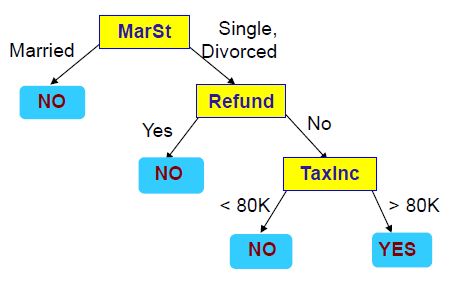
\includegraphics[scale=0.6]{qcm1_tree}    
\end{center}
\begin{center}
    \begin{tabular}{ |c|c|c||c| }
        \hline
        Refund & Marital Status & Taxable Income & Cheat \\
        \hline
        Yes & Single & 220K & No \\
        \hline
        No & Divorced & 75K & No \\
        \hline
        Yes & Single & 70K & Yes \\
        \hline
        No & Married & 110K & No \\
        \hline
        No & Divorced & 81K & No \\
        \hline
        No & Married & 120K & No \\
        \hline
        Yes & Married & 115K & Yes \\
        \hline
        No & Divorced & 145K & Yes \\
        \hline
    \end{tabular}
\end{center}
Answers:
\begin{enumerate}
    \item $\text{accuracy} = \frac{5}{8}$ \textdagger
    \item $\text{accuracy} = \frac{4}{8}$
    \item $\text{accuracy} = \frac{3}{8}$
    \item $\text{accuracy} = 0.375$
\end{enumerate}
\subsection{2\textsuperscript{nd} MCQ}
This question checks if the student knows how to read and use a table of values for the $\chi^2$ test.
Q: During the learning phase of a decision tree, a node is split in 4 child nodes. We decide 
whether to prune it or not with the $\chi^2$ test, with a confidence level of $95\%$.
\\
What should at least be the value of $\Delta$ to not prune the node ?
\\
You may use this value table of the $\chi^2$ distribution.
\\
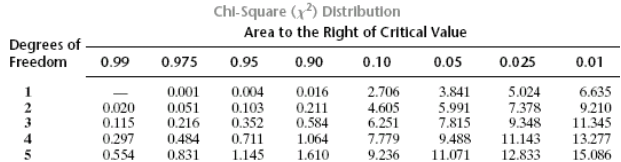
\includegraphics[scale=0.75]{chi2}
\\
Answers:
\begin{enumerate}
    \item 0.352
    \item 0.711
    \item 7.815 \textdagger
    \item 9.488 


\end{enumerate}
\end{document}
